\chapter{Design, implementation, and evaluation}
\label{chapter:design}

This chapter delves deep into the design and implementation of GecWeb, detailing the system's architecture and user interface.

\section{Architecture design}

To make GecWeb more modular, the three-tier architecture, also known as the Model-View-Controller (MVC) architecture, is chosen.
Three-tier architecture is a well-established software application architecture that organizes applications into three logical and physical computing tiers: the presentation tier, or user interface; the application tier, where data is processed; and the data tier, where application data is stored and managed.

The chief benefit of the three-tier architecture is that because each tier runs on its own infrastructure, each tier can be developed simultaneously by a separate development team.
It can be updated or scaled as needed without impacting the other tiers.

\begin{enumerate}
  \item The presentation tier is the user interface and communication layer of the application, where the end user interacts with the application.
        Its main purpose is to display information to and collect information from the user.
        This top-level tier can run on a web browser, as a desktop application, or a graphical user interface (GUI), for example.

  \item The application tier, also known as the logic tier or middle tier, is the heart of the application.
        This tier is responsible for processing user input, making logical decisions, and interacting with the data tier.
        It can also add, delete, or modify data in the data tier.

  \item The data tier is the storage layer of the application, where data is stored, retrieved, and managed.
        This tier can consist of databases, file systems, or other data storage mechanisms.
        The data tier is responsible for managing the application's data and ensuring data integrity and security.
\end{enumerate}

In a three-tier application, all communication goes through the application tier.
The presentation tier and the data tier cannot communicate directly with one another.
Apply this architecture to GecWeb:

\begin{enumerate}
  \item Presentation Layer: The web interface built using Flask and Bootstrap resides in this layer.
  \item It is responsible for rendering the input text box, output text box, and correction highlights.
  \item Application Layer: The Flask RESTful API acts as the controller, handling user requests, managing the selection of GEC models, and coordinating the combination methods.
  \item Data Layer: Although no database is used in GecWeb, the GEC models and combination methods are considered part of the data layer in the context of the three-tier architecture.
        It handles the interaction with the underlying GEC systems and ensures that the corrected text is returned to the application layer.
        The GEC models (GECToR-Bert, GECToR XLNet, GECToR Roberta) and combination methods (ESC, MEMT) reside in this layer.
\end{enumerate}

Although both the GEC models and the web interface can be hosted on the same server, separating them enhances modularity and scalability: the GEC models are hosted on a GPU-powered server, allowing the web interface to run on a CPU-focused server.

\section{Detailed design}

\subsection{System Design and Implementation}

\begin{figure}[htbp]
  \begin{center}
    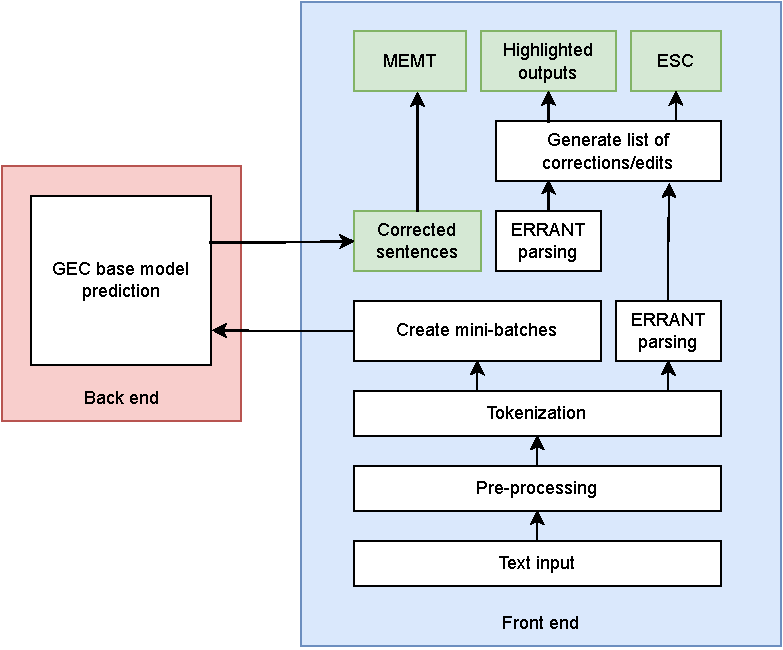
\includegraphics[width=0.7\textwidth]{flowchart}
  \end{center}
  \caption{The process flow of GecWeb}\label{fig:flowchart}
\end{figure}

The process flow of GecWeb is described in Figure~\ref{fig:flowchart}.
All inputs are first split by line and segmented into sentences.
The line index for each sentence is recorded to retain the text structure in the output.
Then, the web interface tokenizes the sentences and combines them into mini-batches to be sent to the base models' API.
If the user chooses to highlight the corrections or combine multiple
base models with ESC, the web interface will also use ERRANT to parse the input sentences.
After receiving the output sentences from each base model, the interface will then parse the base models and outputs using ERRANT if the user chooses to highlight corrections or use ESC.
If not, the outputs are sent to MEMT if the user chooses to combine the models with MEMT.
Otherwise, the output sentences are directly detokenized.
Detokenization also applies to the combination method's output if the user selects more than one base model.

\subsection{User interface design}

The user interface of GecWeb is designed to be responsive and accessible across various screen resolutions, ensuring a seamless experience for users on different devices.
The layout adapts to screens as small as 320x480 pixels, commonly found on mobile phones, up to 1920x1080 pixels, which is standard for desktop monitors.
To maintain accessibility, the color scheme adheres to a contrast ratio above 4.5:1, ensuring readability for users with visual impairments.

Consistency and standardization are key aspects of the interface design.
Buttons maintain a uniform appearance with rounded corners and consistent padding, providing a visually appealing and user-friendly experience.
The "Run" button, which triggers the grammatical error correction process, is prominently displayed in a contrasting color, making it easily identifiable.
Feedback messages, including error notifications and success confirmations, appear at the top of the screen, ensuring they are immediately visible to users.

The color scheme follows a clean and intuitive design, primarily using shades of blue, green, and white.
Corrections made to the text are highlighted in green to enhance visibility, allowing users to easily identify the suggested changes.
This structured approach to design improves usability, ensuring that the interface remains simple, effective, and accessible to a wide range of users.

\section{Application Building}

\subsection{Libraries and Tools}

Table~\ref{tab:tools} provides a comprehensive list of all the tools and libraries that I have used in the development of GecWeb, along with their versions and URLs for more information.

\begin{sidewaystable}[htbp]
  \caption{Tools and libraries}\label{tab:tools}
  \raggedleft
  \begin{tabular}{|l|l|l|l|}
    \hline
    Name             & Purpose                                & Version     & URL                                                 \\ \hline
    WSL              & Linux environment                      & 2.3.26.0    & \url{https://learn.microsoft.com/en-us/windows/wsl} \\ \hline
    Neovim           & Text editor/IDE                        & 0.10.3      & \url{https://github.com/neovim/neovim}              \\ \hline
    Conda            & Package, environment management system & 24.7.1      & \url{https://anaconda.org/anaconda/conda}           \\ \hline
    Python           & Programming language                   & 3.10.16     & \url{https://github.com/python/cpython}             \\ \hline
    Pyright          & Static Type Checker for Python         & 1.1.391     & \url{https://github.com/microsoft/pyright}          \\ \hline
    Ruff             & Linter and formatter for Python        & 0.8.4       & \url{https://github.com/astral-sh/ruff}             \\ \hline
    Pytest           & Unit test frameworks                   & 8.3.4       & \url{https://github.com/pytest-dev/pytest}          \\ \hline
    Curl             & Test API endpoints                     & 8.11.1      & \url{https://github.com/curl/curl}                  \\ \hline
    Windows Terminal & Terminal                               & 1.21.3231.0 & \url{https://github.com/microsoft/terminal}         \\ \hline
    Tmux             & Terminal Multiplexer                   & 3.5a        & \url{https://github.com/tmux/tmux}                  \\ \hline
    Git              & Version control system                 & 2.45.2      & \url{https://git-scm.com}                           \\ \hline
    Docker           & Containerization and Virtualization    & 24.7.0      & \url{https://www.docker.com}                        \\ \hline
    Flask            & Web Framework                          & 3.1.0       & \url{https://flask.palletsprojects.com}             \\ \hline
    Bootstrap        & Front-End                              & 5.2.3       & \url{https://getbootstrap.com}                      \\ \hline
    Gradio           & Front-End                              & 3.20.1      & \url{https://github.com/gradio-app/gradio}          \\ \hline
    ERRANT           & Extract/classify grammatical errors    & 2.3.3       & \url{https://github.com/chrisjbryant/errant}        \\ \hline
    NLTK             & Pre/Post processing data               & 3.9.1       & \url{https://github.com/nltk/nltk}                  \\ \hline
    SpaCy            & Natural Language Processing            & 2.3.9       & \url{https://github.com/explosion/spaCy}            \\ \hline
  \end{tabular}
\end{sidewaystable}

WSL (Windows Subsystem for Linux) was used to provide a Linux-like development environment on Windows.
Since many machine learning tools and deployment workflows are optimized for Linux, WSL allows for a smooth experience without needing a separate Linux machine or virtual machine.

Neovim was selected as the primary code editor due to its speed, extensibility, and lightweight nature.
With proper configurations, Neovim offers an efficient development experience, particularly when working within a terminal-based environment like WSL.

Conda was used for managing Python environments and dependencies.
Given that machine learning projects often require specific versions of libraries to maintain compatibility, Conda provided a structured way to manage these dependencies without interfering with system-wide Python installations.
This ensured a reproducible environment across different machines, and different projects.

Pyright was used as a static type checker to ensure type safety in Python code.
Since Python is dynamically typed, it can sometimes lead to runtime errors that are hard to catch during development.
Pyright helped enforce type annotations, making the code more maintainable and reducing the likelihood of bugs.

Ruff was employed as a linter and code formatter to maintain coding standards and improve code quality.
It offers fast performance and supports multiple linting rules, ensuring consistency across the codebase.
Using Ruff also helped in catching potential issues early in development.

Windows Terminal provided a modern and customizable terminal experience on Windows.
With support for multiple profiles and tabs, it allowed for a smooth workflow when working with WSL, Git, and various command-line tools simultaneously.

Tmux was used as a terminal multiplexer, enabling multiple terminal sessions within a single window.
This was particularly useful when running long-running processes such as model training, debugging, and managing multiple environments simultaneously.
It ensured that sessions remained active even when disconnected from a remote server.

Git was an essential tool for version control and collaboration.
It enabled efficient tracking of changes, managing branches, and synchronizing work across different devices.
With Git, the project remained organized, and it was easier to roll back changes if needed.

Docker was used for containerization and deployment.
Since machine learning applications often have complex dependencies, Docker ensured that GecWeb could be packaged and deployed in a consistent and reproducible environment.
This was especially useful when deploying the application to cloud servers or sharing the setup with other developers.

Python, Flask, Bootstrap, Gradio, ERRANT, NLTK and SpaCy were already discussed in Chapter~\ref{chapter:methodology}, therefore I will not discuss them here.

\subsection{First prototype}

As mentioned in Chapter~\ref{chapter:requirement}, Gradio was used to build the first protype of GecWeb.
The user interface of this prototype is shown in Figure~\ref{fig:prototype}.

\begin{figure}[htbp]
  \begin{center}
    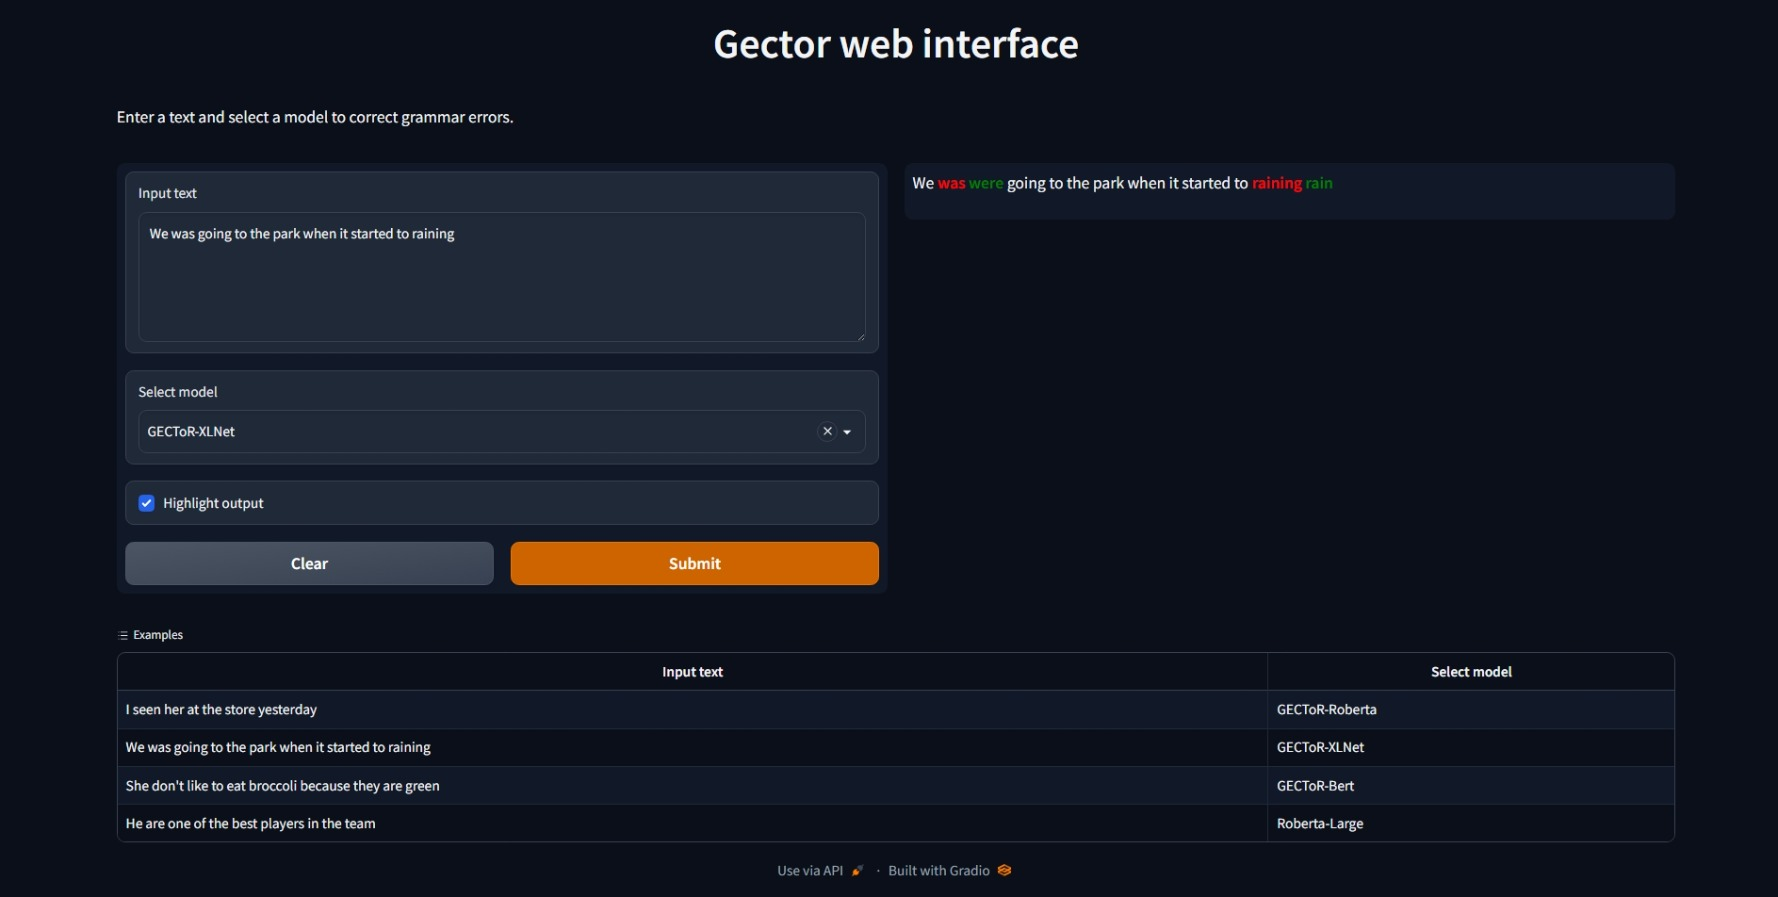
\includegraphics[width=\textwidth]{prototype}
  \end{center}
  \caption{First prototype of GecWeb}\label{fig:prototype}
\end{figure}

In this prototype, the system combination method is not yet implemented.
Additionally, both the models and the interface is run in the same machine.
Although it lack some functionality that I specified in Chapter~\ref{chapter:requirement}, it provides a quick demo of GecWeb.
You can still access this version on \href{https://huggingface.co/spaces/canh25xp/gector_demo}{My Hugging Face page}
To save resources, the app auto put it self to sleep after 24 hours of inactivity.
So you might have to wait for 10-20s for the app to boot up.

\subsection{Illustration of GecWeb}

The interface of GecWeb consists of five components, which are (i) base model selection, (ii) combination method selection, (iii) output mode, (iv) input text box, and (v) output text box.
The user interface of GecWeb is shown in Figure~\ref{fig:home}.
You might notice that GecWeb bears some resemblance to Google Translate, with the app name at the top, an input box on the left, and an output box on the right.
This similarity is because GecWeb's design is heavily inspired by Google Translate, given that both applications perform text-to-text transformations.

\begin{figure}[htbp]
  \begin{annotatedFigure}
    {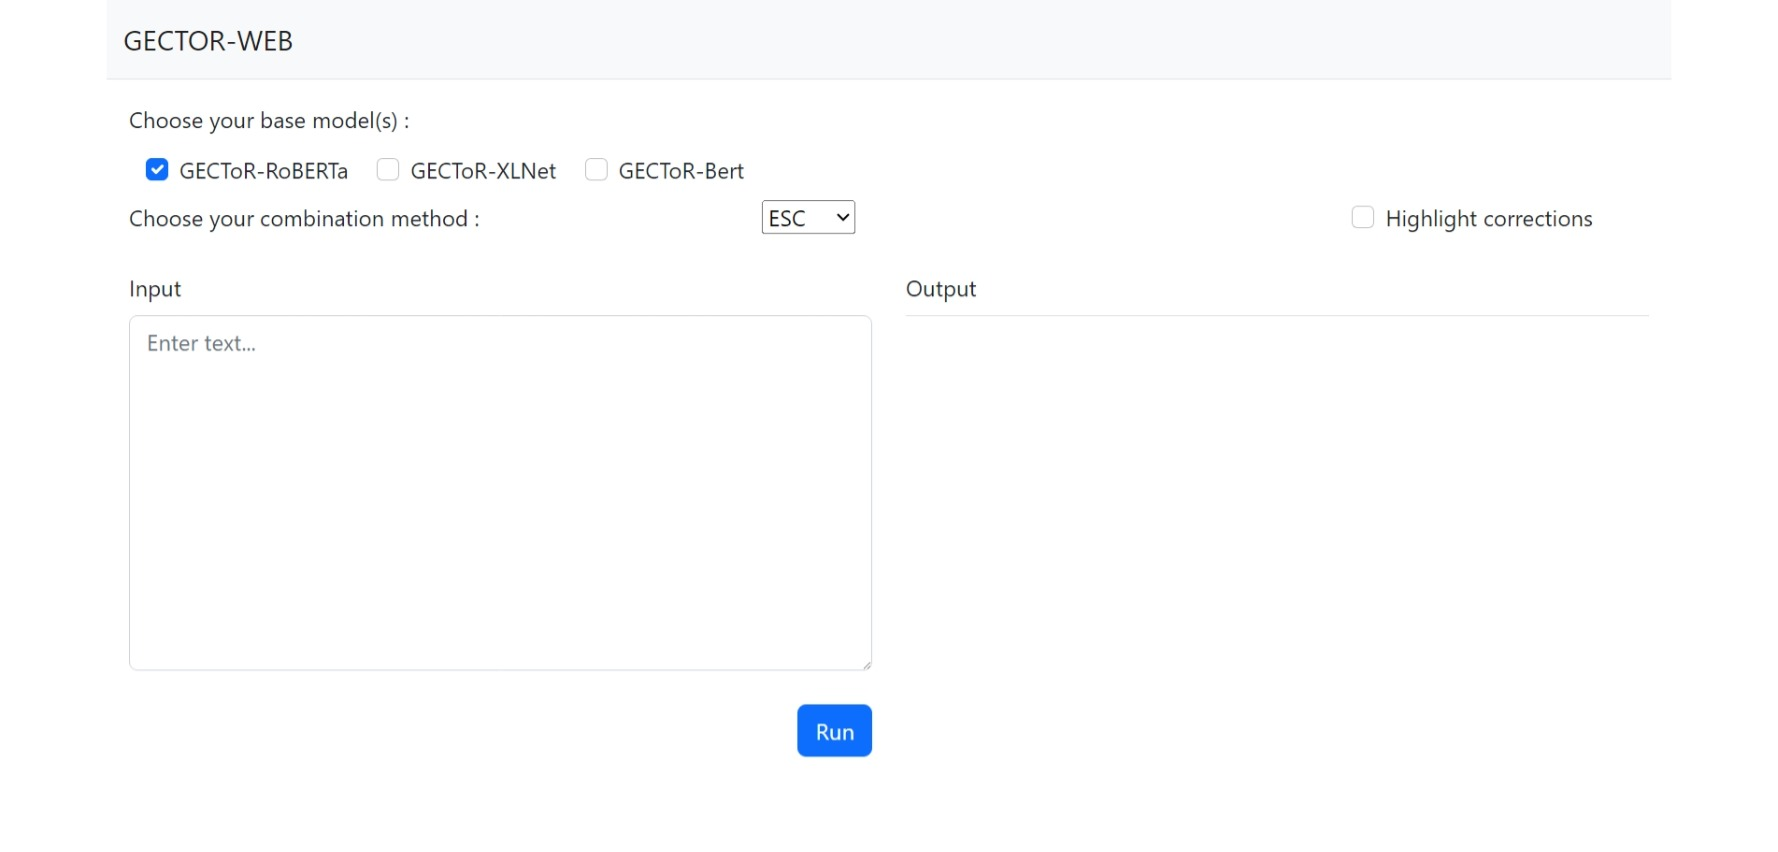
\includegraphics[width=\textwidth]{home}}
    \annotatedFigureBox{0.0905,0.7727}{0.4305,0.8393}{i}{0.4305,0.8393}%tr
    \annotatedFigureBox{0.434,0.7266}{0.5105,0.8003}{ii}{0.5105,0.8003}%tr
    \annotatedFigureBox{0.7615,0.7308}{0.9195,0.7934}{iii}{0.9195,0.7934}%tr
    \annotatedFigureBox{0.1285,0.3489}{0.4595,0.6243}{iv}{0.4595,0.6243}%tr
    \annotatedFigureBox{0.574,0.2591}{0.8665,0.6118}{v}{0.8665,0.6118}%tr
  \end{annotatedFigure}
  \caption{The User Interface of GecWeb.}\label{fig:home}
\end{figure}

\subsubsection{Base Model Selection}

The user first needs to choose the base model(s).
If the user chooses more than one base model, GecWeb will run a system combination method based on the combination method selected, as described in Chapter 3.

\subsubsection{Combination Method Selection}

Next, the user needs to choose the combination method.
If the user only chooses one base system, the selected combination method is ignored.
As mentioned earlier in Chapter 3, GecWeb includes two state-of-the-art system combination methods, ESC and MEMT.

\subsubsection{Output Mode}

Users can choose to highlight the corrections by selecting the "Highlight corrections" box.
If the user chooses to highlight the corrections, text spans in the output text that are different from the input text are highlighted in green and a simple explanation of each correction can be displayed by clicking a highlighted text span.
The appearance of highlighted corrections can be seen in Figure~\ref{fig:highlight}.
Displaying corrections with simple explanations can help language learners to understand their mistakes better.
I extracted the corrections with their edit types using ERRANT.

\begin{figure}[htbp]
  \begin{center}
    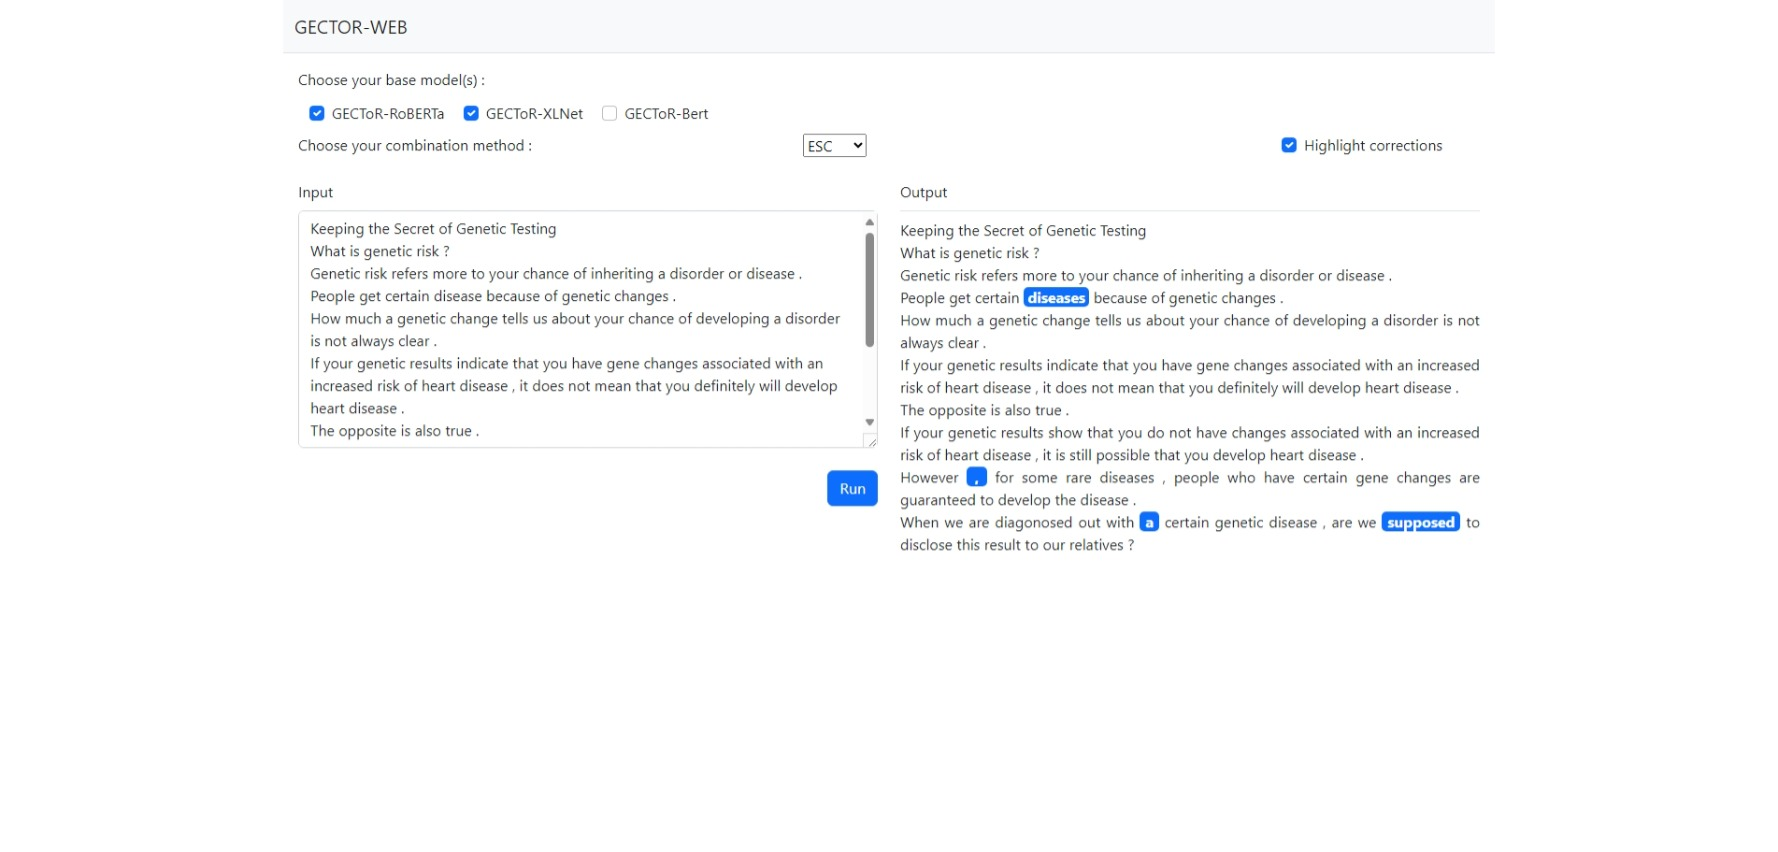
\includegraphics[width=\textwidth]{highlight}
  \end{center}
  \caption{The interface with highlighted corrections, showing green highlights for corrected text and explanations for each correction.}\label{fig:highlight} \end{figure}

\subsubsection{Input Text Box}

The user needs to put the text they want to correct in the input text box and clicks the run button.
The corrected text will then be displayed in the output text box.
Most recent GEC base systems expect the input to be a single sentence tokenized with SpaCy version 1.9, following the requirement from the BEA-2019 shared task.
As such, an input text needs to be segmented into sentences and then tokenized with SpaCy before each sentence is given as the input to the GEC model.
To retain the text structure, it is first split by line before segmented into sentences.
This way, I can keep the information on which line a sentence should be printed.
To segment a text into sentences, I follow the practice used in the NUCLE corpus by using the nltk Punkt
tokenizer.

\subsubsection{Output Text Box}

After a text is entered into the input text box and the "Run" button is clicked, the corrected text will appear in the output text box.
As the base GEC systems are expected to work on tokenized input and output, the output text needs to be detokenized to look more natural.
Since SpaCy does not have a detokenizer and the document context of the original input may no longer be relevant after a sentence is corrected, I use Moses todetokenize a sentence.
I found that Moses can detokenize a sentence that is tokenized by SpaCy reasonably well, only missing some cases like the detokenization of "is n't" and "are n;t" and removing spaces around hyphens.
For these missed cases, I create simple rules to apply string replacement after Moses detokenization.
Detokenization is not applied if the user chooses to highlight the corrections because the highlights need some room to make them clearly visible.

\section{Testing}

\subsection{Back-end Testing}

The back-end contains several test methods, with both automated and manual testing conducted to ensure the correctness and reliability of the system.
The unit tests are implemented using pytest, a popular testing framework in Python.

These tests focus on verifying the behavior of individual components of the back-end, namely:
(i) test bert embedder,
(ii) test gec model,
(iii) test gec predictor,
(iv) test roberta embedder,
(v) test seq2labels,
(vi) test token indexer,
(vii) test tokenization.

The Test Token Embedder for BERT Model ensures that the token embedding process for the BERT model functions correctly, validating that the input text is properly tokenized and converted into embeddings that the model can process.
Similarly, the Test Token Embedder for RoBERTa Model performs the same validation for the RoBERTa model, ensuring compatibility with different transformer-based architectures.
The Test Class for GecModel verifies the core functionality of the grammatical error correction model, including its ability to process input text and generate corrections.
Additionally, the Test Class for Seq2Labels Model ensures that the sequence-to-labels model, which is used for sequence tagging tasks, operates as expected.

In addition to unit tests, regression testing is performed to ensure that changes to the codebase do not introduce unintended side effects.
The regression tests use the GECToR-Roberta model to generate predictions for all test files and verify that there are no changes in the output.
This is particularly important for maintaining the consistency of the system, especially when updates or modifications are made to the models or the back-end logic.
The regression tests help ensure that the system's performance remains stable over time and that any new changes do not degrade the quality of the corrections.

To further streamline the testing process, both the unit tests and regression tests are automated using GitHub Actions in multiple Python environments (3.8, 3.9, and 3.10) to ensure compatibility across different versions.
The tests are triggered automatically whenever code is pushed to the main branch, ensuring continuous integration and preventing faulty code from being merged.

Finally, manual API testing is conducted using curl to interact with the back-end API directly, further confirming the proper functioning of the web service.

\section{Deployment}

The deployment of GecWeb is designed to ensure efficient access to grammatical error correction while leveraging the computing power of GPU-focused servers.
The system consists of two main components: the Gec API, which handles the processing of text corrections, and the Gec Web interface, which provides users with an interactive front end to access the correction features.

The Gec API is hosted on Hugging Face Inference Endpoints, which provide dedicated GPU resources to efficiently run deep learning models.
Since grammatical error correction models, such as GECToR, require significant computational power for inference, deploying the API on GPU-accelerated infrastructure ensures fast response times and scalability.
By hosting the API on Hugging Face Inference Endpoints, the system benefits from automatic scaling, secure deployment, and optimized performance without requiring extensive server management.

The Gec Web interface is hosted separately on Hugging Face Spaces, a platform designed for hosting interactive web applications.
Spaces allow developers to easily deploy front-end applications built with frameworks like Flask and Bootstrap, providing a simple way to share machine-learning models with the public.
Hosting GecWeb on Spaces ensures that users can access the interface without requiring local installations, making the system widely accessible.
The front-end communicates with the Gec API by sending text data for processing and receiving corrected outputs, ensuring a seamless and responsive user experience.

By separating the back-end processing from the front-end interface, the deployment strategy optimizes performance and usability.
The API benefits from high-performance GPUs, while the web interface remains lightweight and accessible through any modern browser.
This cloud-based approach allows for easy updates, maintenance, and potential future expansions, making GecWeb an efficient and user-friendly platform for grammatical error correction.

The correction speed of GecWeb is fast.
Running on an NVIDIA Titan X GPU server with 12GB memory, GECToR Roberta can correct text at a speed of 723 words per second, GECToR XLNet at 640 words per second, and GECToR-Bert at 37 words per second.
Using ESC to combine base systems only adds a small amount of overhead.
For example, using ESC to combine GECToR Roberta and GECToR-Bert can correct text at a speed of 32 words per second, marginally slower than using GECToR-Bert alone.

